\documentclass[pdf]
{beamer}
\mode<presentation>{}
%% preamble

\usepackage{ulem}
%\usepackage{gantt}
\usepackage{tikz}
\usepackage{tikz-qtree}
\usetikzlibrary{shapes}

% Declare background layer
\pgfdeclarelayer{bg}
\pgfsetlayers{bg,main}

\title[ESTEC 2017]
{
    \textbf{Using Concept Graphs for Modelling Robotic Systems}
}
\author{Moritz Schilling}
\date{\today}

\begin{document}

\begin{frame}[plain]
    \titlepage
\end{frame}

%% INTRO %%

\begin{frame}{Different Views on a Robotic System}
    % Processors & Communication Links
    \only<1>{
    \begin{center}
    \begin{tikzpicture}
    \node[align=center] (ROBO) at (0,0) {
        \includegraphics[width=\textwidth]{pics/Charlie.png}
    };

    % Highlight x86
    \node[align=center, fill=red, circle, inner sep=0pt, minimum size=2mm] (X86) at (1.5,2) {
    };

    % Highlight uC
    \node[align=center, fill=blue, inner sep=0pt, minimum size=2mm] (UC1) at (-2.2,-2.2) {
    };
    \node[align=center, fill=blue, inner sep=0pt, minimum size=2mm] (UC2) at (-2.8,-1.5) {
    };
    \node[align=center, fill=blue, inner sep=0pt, minimum size=2mm] (UC3) at (-0.6,-1.4) {
    };
    \node[align=center, fill=blue, inner sep=0pt, minimum size=2mm] (UC4) at (2.3,-1) {
    };
    \node[align=center, fill=blue, inner sep=0pt, minimum size=2mm] (UC5) at (-1.1,1.3) {
    };

    % Highlight FPGA
    \node[align=center, fill=olive, diamond, inner sep=0pt, minimum size=3mm] (FPGA1) at (1,2) {
    };
    \node[align=center, fill=olive, diamond, inner sep=0pt, minimum size=3mm] (FPGA2) at (0.7,1.9) {
    };
    \node[align=center, fill=olive, diamond, inner sep=0pt, minimum size=3mm] (FPGA3) at (1.2,1.2) {
    };
    \node[align=center, fill=olive, diamond, inner sep=0pt, minimum size=3mm] (FPGA4) at (-1,0.2) {
    };

    % Connections
    \draw[-, thick] (X86) -- (FPGA1) -- (FPGA2) -- (FPGA3) -- (FPGA4) -- (UC3);

    % Legend
    \node[align=center, red] (LX86) at (5,4) {
        x86
    };
    \draw[->, red] (LX86) -| (X86);
    \node[align=center, blue] (LUC) at (5,-3) {
        $\mu$C
    };
    \draw[->, blue] (LUC) -| (UC1);
    \draw[->, blue] (LUC) -| (UC2);
    \draw[->, blue] (LUC) -| (UC3);
    \draw[->, blue] (LUC) -| (UC4);
    \draw[->, blue] (LUC) -| (UC5);
    \node[align=center, olive] (LFPGA) at (-5,4) {
        FPGA
    };
    \draw[->, olive] (LFPGA) |- (FPGA1);
    \draw[->, olive] (LFPGA) |- (FPGA2);
    \draw[->, olive] (LFPGA) |- (FPGA3);
    \draw[->, olive] (LFPGA) |- (FPGA4);

\end{tikzpicture}

    \end{center}
    }
    % Joints & Links/Bodies
    \only<2>{
    \begin{center}
    \begin{tikzpicture}
    \node[align=center] (ROBO) at (0,0) {
        \includegraphics[width=\textwidth]{pics/Charlie.png}
    };
    
    % Show joints
    \node[align=center, fill=red, circle, inner sep=0pt, minimum size=2mm] (FR1) at (1,2) {
    };
    \node[align=center, fill=red, circle, inner sep=0pt, minimum size=2mm] (FR2) at (0.7,1.9) {
    };
    \node[align=center, fill=red, circle, inner sep=0pt, minimum size=2mm] (FR3) at (1.2,1.2) {
    };
    \node[align=center, fill=red, circle, inner sep=0pt, minimum size=2mm] (FR4) at (-1,0.3) {
    };
    \node[align=center] (FR5) at (-0.6,-1.8) {};
   
    \node[align=center, fill=red, circle, inner sep=0pt, minimum size=2mm] (RR1) at (-2,1.7) {
    };
    \node[align=center, fill=red, circle, inner sep=0pt, minimum size=2mm] (RR2) at (-2.4,1.6) {
    };
    \node[align=center, fill=red, circle, inner sep=0pt, minimum size=2mm] (RR3) at (-3,1.4) {
    };
    \node[align=center, fill=red, circle, inner sep=0pt, minimum size=2mm] (RR4) at (-1.5,-0.3) {
    };
    \node[align=center, fill=red, diamond, inner sep=0pt, minimum size=2mm] (RR5) at (-2.8,-1.8) {
    };
    
    
    \node[align=center, fill=red, inner sep=0pt, minimum size=2mm] (SPINE) at (-0.5,2) {
    };
    

	% Show links
	\draw[-, thick] (SPINE) -- (FR1) -- (FR2) -- (FR3) -- (FR4) -- (FR5);
	\draw[-, thick] (SPINE) -- (RR1) -- (RR2) -- (RR3) -- (RR4) -- (RR5);    
    
\end{tikzpicture}

    \end{center}
    }
\end{frame}
\begin{frame}{DROCK}
    \centering
    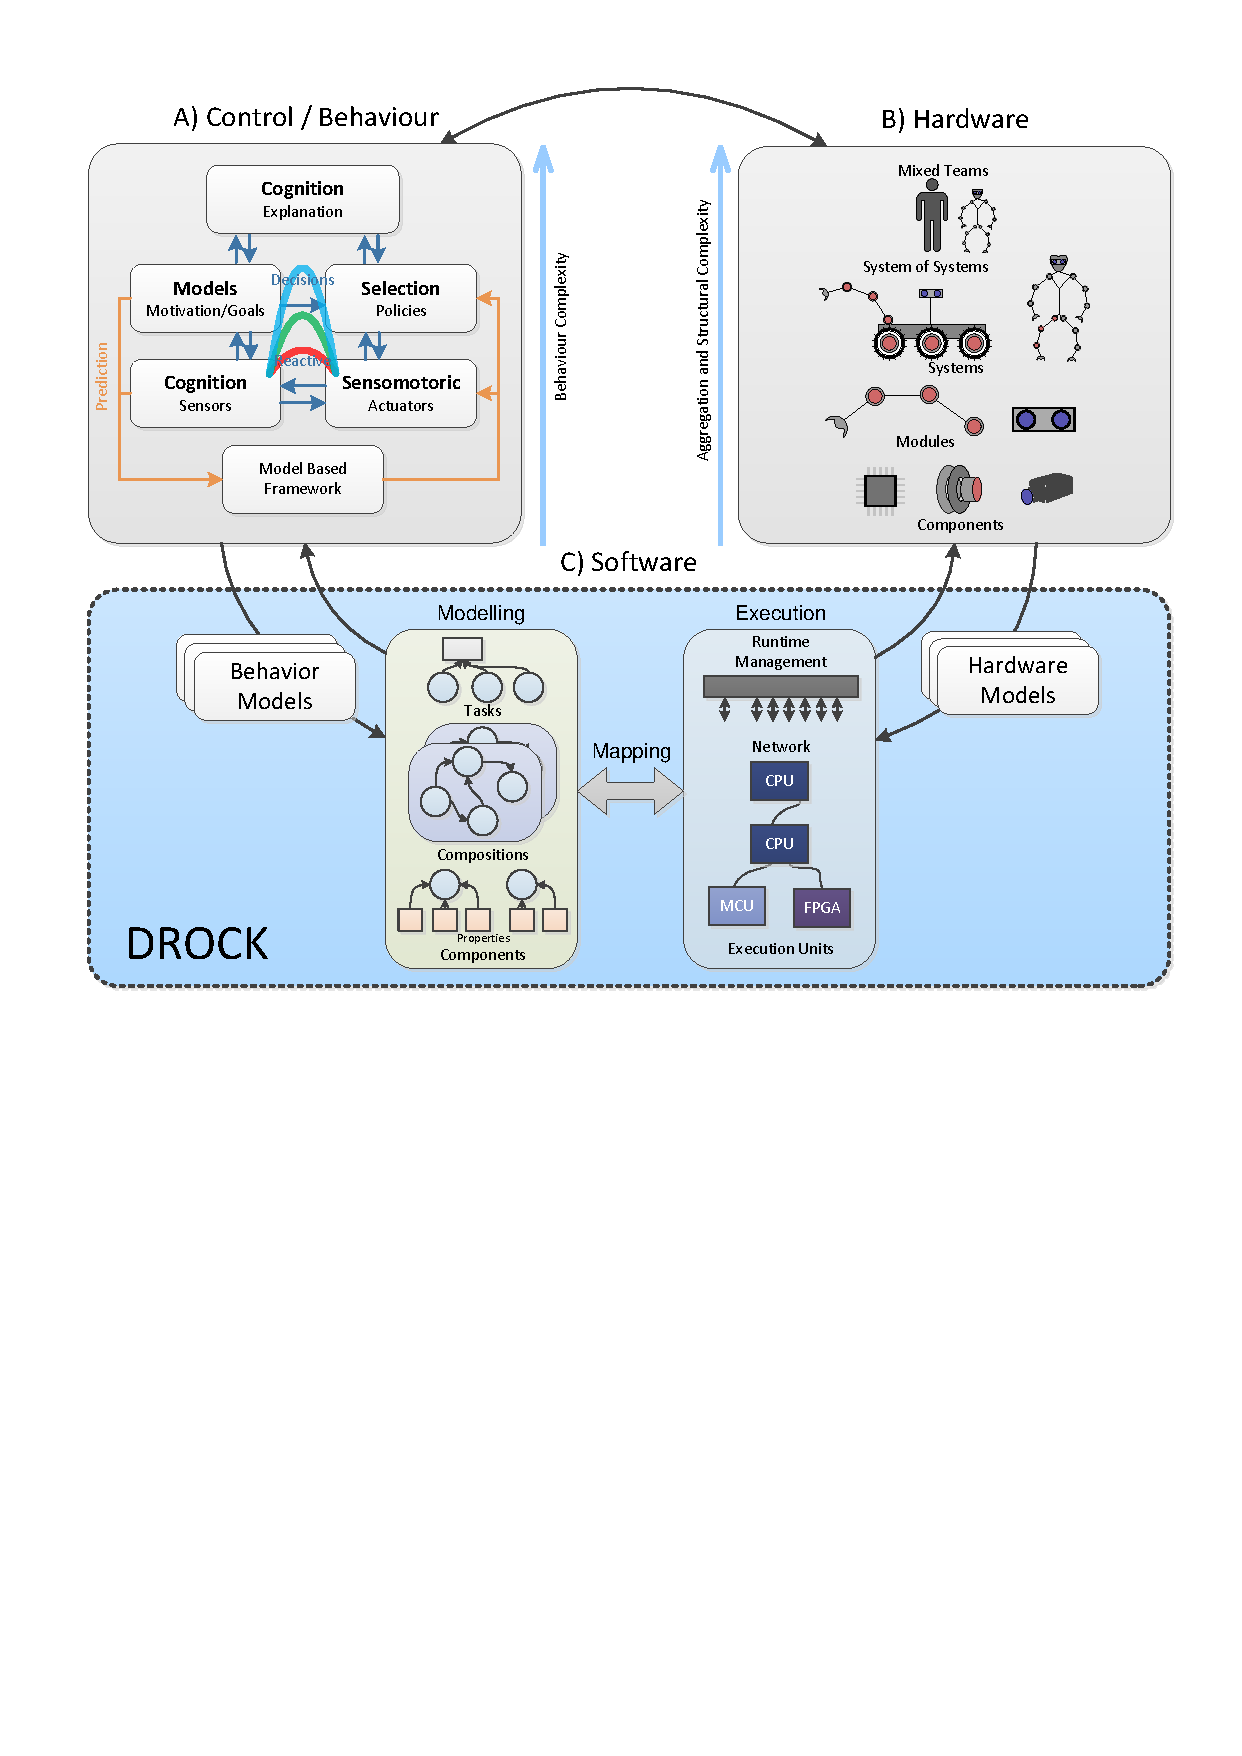
\includegraphics[width=.9\textwidth]{pics/circle.pdf}
\end{frame}

\begin{frame}{Motivation}
    %WHAT DO YOU WANT TO DO AND WHY?
	\centering
	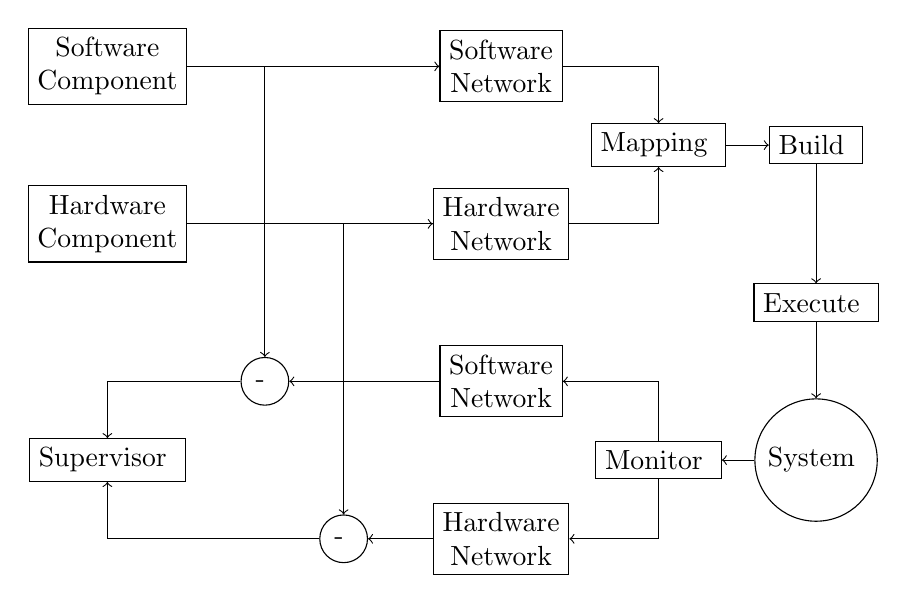
\begin{tikzpicture}
        \node[draw, align=center] (SWCOMP) at (0,1) {
            Software\\Component
        };
        \node[draw, align=center] (HWCOMP) at (0,-1) {
            Hardware\\Component
        };
        \node[draw, align=center] (SWNET) at (5,1) {
            Software\\Network
        };
        \node[draw, align=center] (HWNET) at (5,-1) {
            Hardware\\Network
        };
        \node[draw, align=center] (MAP) at (7,0) {
            Mapping
        };
        \node[draw, align=center] (BUILD) at (9,0) {
            Build
        };
        \node[draw, align=center] (EXEC) at (9,-2) {
            Execute
        };
        \node[circle, draw, align=center] (SYS) at (9,-4) {
            System
        };
        \node[draw, align=center] (MON) at (7,-4) {
            Monitor
        };
        \node[draw, align=center] (SWNET2) at (5,-3) {
            Software\\Network
        };
        \node[draw, align=center] (HWNET2) at (5,-5) {
            Hardware\\Network
        };
        \node[circle, draw, align=center] (SWDIFF) at (2,-3) {
            -
        };
        \node[circle, draw, align=center] (HWDIFF) at (3,-5) {
            -
        };
        \node[draw, align=center] (SUPERVISOR) at (0,-4) {
            Supervisor
        };
        \draw[->] (SWNET) -| (MAP);
        \draw[->] (HWNET) -| (MAP);
        \draw[->] (MAP) -- (BUILD);
        \draw[->] (BUILD) -- (EXEC);
        \draw[->] (EXEC) -- (SYS);
        \draw[->] (SYS) -- (MON);
        \draw[->] (MON) |- (SWNET2);
        \draw[->] (MON) |- (HWNET2);
        \draw[->] (SWNET) -| (SWDIFF);
        \draw[->] (SWNET2) -- (SWDIFF);
        \draw[->] (HWNET) -| (HWDIFF);
        \draw[->] (HWNET2) -- (HWDIFF);
        \draw[->] (SWDIFF) -| (SUPERVISOR);
        \draw[->] (HWDIFF) -| (SUPERVISOR);
        \draw[->] (SWCOMP) -- (SWNET);
        \draw[->] (HWCOMP) -- (HWNET);
\end{tikzpicture}

\end{frame}

%% THEORY %%

\begin{frame}{Generalized Hypergraph}
	\begin{columns}
		\begin{column}{.5\textwidth}
			\begin{description}
			\item[Graph] Two nodes can be connected by an edge
			\item[Hypergraph] An edge can connect arbitrary many nodes
			\item[Generalized Hypergraph] An edge can also point to another edge
			\end{description}
		\end{column}
		\begin{column}{.5\textwidth}
			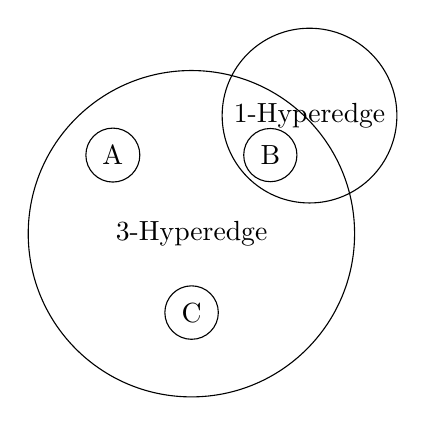
\begin{tikzpicture}
		%\node[draw, align=center] (HEDGE_E) at (-2,2) {
        %    4-Hyperedge
        %};
		%\node[draw, align=center] (HEDGE_D) at (6,0) {
        %    1-Hyperedge
        %};
        %\node[draw, align=center] (HEDGE_A) at (2,0) {
        %    2-Hyperedge
        %};
        %\node[draw, align=center] (HEDGE_B) at (-2,-2) {
        %    0-Hyperedge
        %};
        %\node[draw, align=center] (HEDGE_C) at (6,-2) {
        %    0-Hyperegde
        %};
        %\draw[->, very thick] (HEDGE_A) to (HEDGE_B);
        %\draw[->, very thick] (HEDGE_A) to (HEDGE_C);
        %\draw[->, very thick] (HEDGE_D) to (HEDGE_C);
        %\draw[->, very thick] (HEDGE_E) to (HEDGE_A);
        %\draw[->, very thick] (HEDGE_E) to (HEDGE_B);
        %\draw[->, very thick] (HEDGE_E) to (HEDGE_C);
        %\draw[->, very thick] (HEDGE_E) to (HEDGE_D);
        \node[matrix, circle, draw] (HEDGE_C) at (0,0) {
        	\node[draw,circle] (HEDGE_A) at (-1,0.5) {A};
        	\node[draw,circle] (HEDGE_B) at (1,0.5) {B};
        	\node[] (label) at (0,-0.5) {3-Hyperedge};
        	\node[draw,circle] (HEDGE_F) at (0,-1.5) {C};\\
        };
        \node[draw,circle] (HEDGE_D) at (1.5,1.5) {
        	1-Hyperedge
        };
\end{tikzpicture}
			% Nodes are just special 0-Hyperedges!
		\end{column}
	\end{columns}
\end{frame}

\begin{frame}{Conceptual Graphs}
    \begin{description}
        \item[Concept] represents things like classes, elements, objects etc.
        \item[Relation] encodes the semantics between different concepts.
    \end{description}
    \begin{itemize}
        \item Encoding concepts as nodes and relation as edges ($Cat - isA \to Animal$)
        \item For N-ary relations you want hyperedges ($Cat - isA \to Animal, Pet$)
        \item For relations over relations you want generalized hyperedges ($X - follows* \to Y, follows* - by \to Car$) 
    \end{itemize}
\end{frame}


\begin{frame}{Domain Overview}
    % TODO: Here a nice pic on the right would be nice?
    \begin{itemize}
        \item Generalized Hypergraph
        \item Concept Graph
        \item Common Concept Graph
        \item Hardware Domain Graph
        \begin{itemize}
            \item Computational Hardware
            \item Electronics
            \item Mechanics/Kinematics
        \end{itemize}
        \item Software Domain Graph
        \begin{itemize}
            \item Behaviors
            \item Algorithms
            \item Implementations
        \end{itemize}
    \end{itemize}
\end{frame}

\begin{frame}{Implementation}
    \begin{description}
    \item[Hyperedge] as an id, a string and a vector of sets of unique ids (incidence list)
    \item[Hypergraph] as a list of hyperedges belonging to that graph
    \item[Concept Graph] as having two predefined hyperedges encoding \emph{concepts} and \emph{relations}
    \item[Common Concept Graph] defining predefined relations for
        \begin{itemize}
        \item type hierarchies (also for relations!) %IS-A, SUBREL-OF
        \item individuals \& facts % INSTANCE-OF, FACT-OF
        \item aggregation %HAS-A
        \item composition %PART-OF
        \item topology %CONNECTS
        \end{itemize}
    \end{description}
\end{frame}

\begin{frame}{Algorithm Domain}
	\centering
	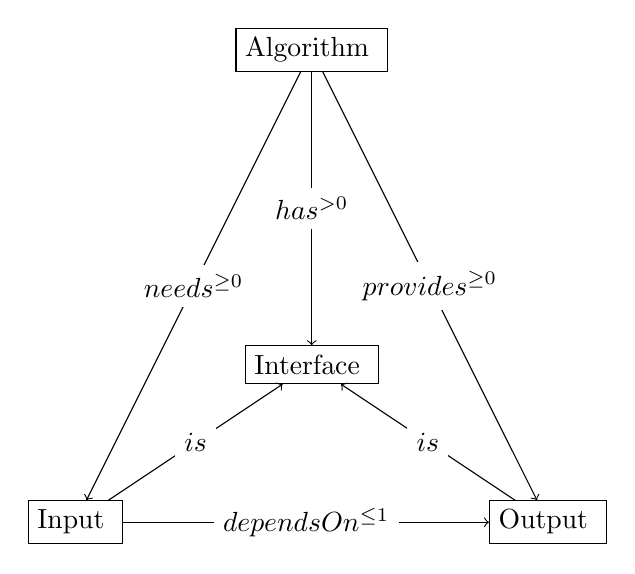
\begin{tikzpicture}
        \node[draw, align=center] (Algorithm) at (0,3) {
            Algorithm
        };
        \node[draw, align=center] (Interface) at (0,-1) {
            Interface
        };
        \node[draw, align=center] (Input) at (-3,-3) {
            Input
        };
        \node[draw, align=center] (Output) at (3,-3) {
            Output
        };
        \draw[->] (Algorithm) to node[fill=white] {
            $has^{>0}$
        } (Interface);
        \draw[->] (Algorithm) to node[fill=white] {
            $needs^{\geq 0}$
        } (Input);
        \draw[->] (Algorithm) to node[fill=white] {
            $provides^{\geq 0}$
        } (Output);
        \draw[->] (Input) to node[fill=white] {
            $is$
        } (Interface);
        \draw[->] (Output) to node[fill=white] {
            $is$
        } (Interface);
        \draw[->] (Input) to node[fill=white] {
            ${dependsOn^{\leq 1}}$
        } (Output);
\end{tikzpicture}
\end{frame}

\begin{frame}{Algorithm Class}
	\centering
	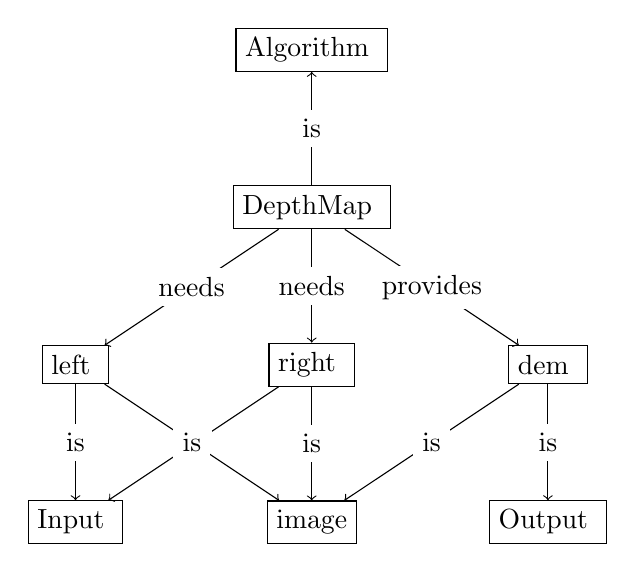
\begin{tikzpicture}[remember picture]
		\node[draw, align=center] (DepthMap) at (0,0) {
			DepthMap
		};
        \node[draw, align=center] (Algorithm) at (0,2) {
            Algorithm
        };
        \node[draw, align=center] (left) at (-3,-2) {
        	left
        };
        \node[draw, align=center] (right) at (0,-2) {
        	right
        };
        \node[draw, align=center] (dem) at (3,-2) {
        	dem
        };
        \node[draw, align=center] (Input) at (-3,-4) {
        	Input
        };
        \node[draw, align=center] (Output) at (3,-4) {
        	Output
        };
        \node[draw] (Interface) at (0,-4) {
        	image
        };
        \draw[->] (DepthMap) to node[fill=white] { is } (Algorithm);
        \draw[->] (DepthMap) to node[fill=white] { needs } (left);
        \draw[->] (DepthMap) to node[fill=white] { needs } (right);
        \draw[->] (DepthMap) to node[fill=white] { provides } (dem);
        \draw[->] (left) to node[fill=white] {is} (Input);
        \draw[->] (right) to node[fill=white] {is} (Input);
        \draw[->] (dem) to node[fill=white] {is} (Output);
        \draw[->] (left) to node[fill=white] {is} (Interface);
        \draw[->] (right) to node[fill=white] {is} (Interface);
        \draw[->] (dem) to node[fill=white] {is} (Interface);
\end{tikzpicture}
\end{frame}

\begin{frame}{Algorithm Network}
	\centering
	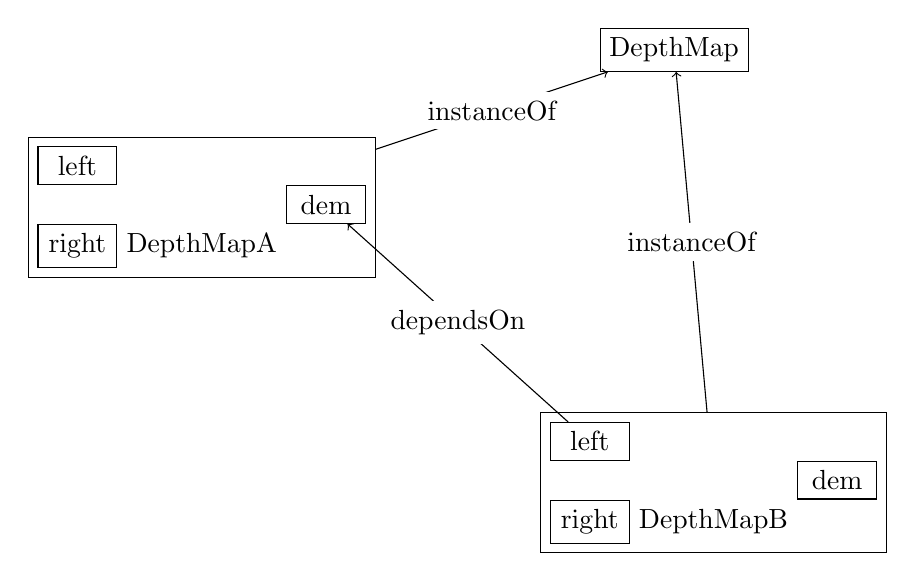
\begin{tikzpicture}[remember picture]
		\node[draw] (DepthMap) at (3,3) {
			DepthMap
		};
		\node[matrix, draw] (DepthMapA) at (-3,1) {
			\node[draw, minimum width=1cm] (left) {left}; & & \\
			& & \node[draw, minimum width=1cm] (demA) {dem}; \\
			\node[draw, minimum width=1cm] (right) {right}; & \node (label) {DepthMapA}; & \\
		};
		\node[matrix, draw] (DepthMapB) at (3.5,-2.5) {
			\node[draw, minimum width=1cm] (leftB) {left}; & & \\
			& & \node[draw, minimum width=1cm] (dem) {dem}; \\
			\node[draw, minimum width=1cm] (right) {right}; & \node (label) {DepthMapB}; & \\
		};
		\draw[->] (DepthMapA) to node[fill=white] {instanceOf} (DepthMap);
		\draw[->] (DepthMapB) to node[fill=white] {instanceOf} (DepthMap);
		\draw[->] (leftB) to node[fill=white] {dependsOn} (demA);
\end{tikzpicture}
\end{frame}

%\begin{frame}{Hierarchy}
%	\begin{itemize}
%		\item $(* \to *')$ labelled hyperedge $*$ pointing to other hyperedge $*'$
%		\item $(Concept \to *)$ $*$ represents a concept
%		\item $(Relation \to *)$ $*$ represents a relation
%		\item $(A - R \to B)$ $A$ is $R$-related to $B$
%		\item Domain specification (Domain of Animals)
%		\item Class specification ($Dog - isA \to Animal$)
%		\item Object specification ($Bello - instanceOf \to Dog$)
%	\end{itemize}
%\end{frame}


%% RESULTS %%

\begin{frame}{HypergraphGUI}
    \centering
    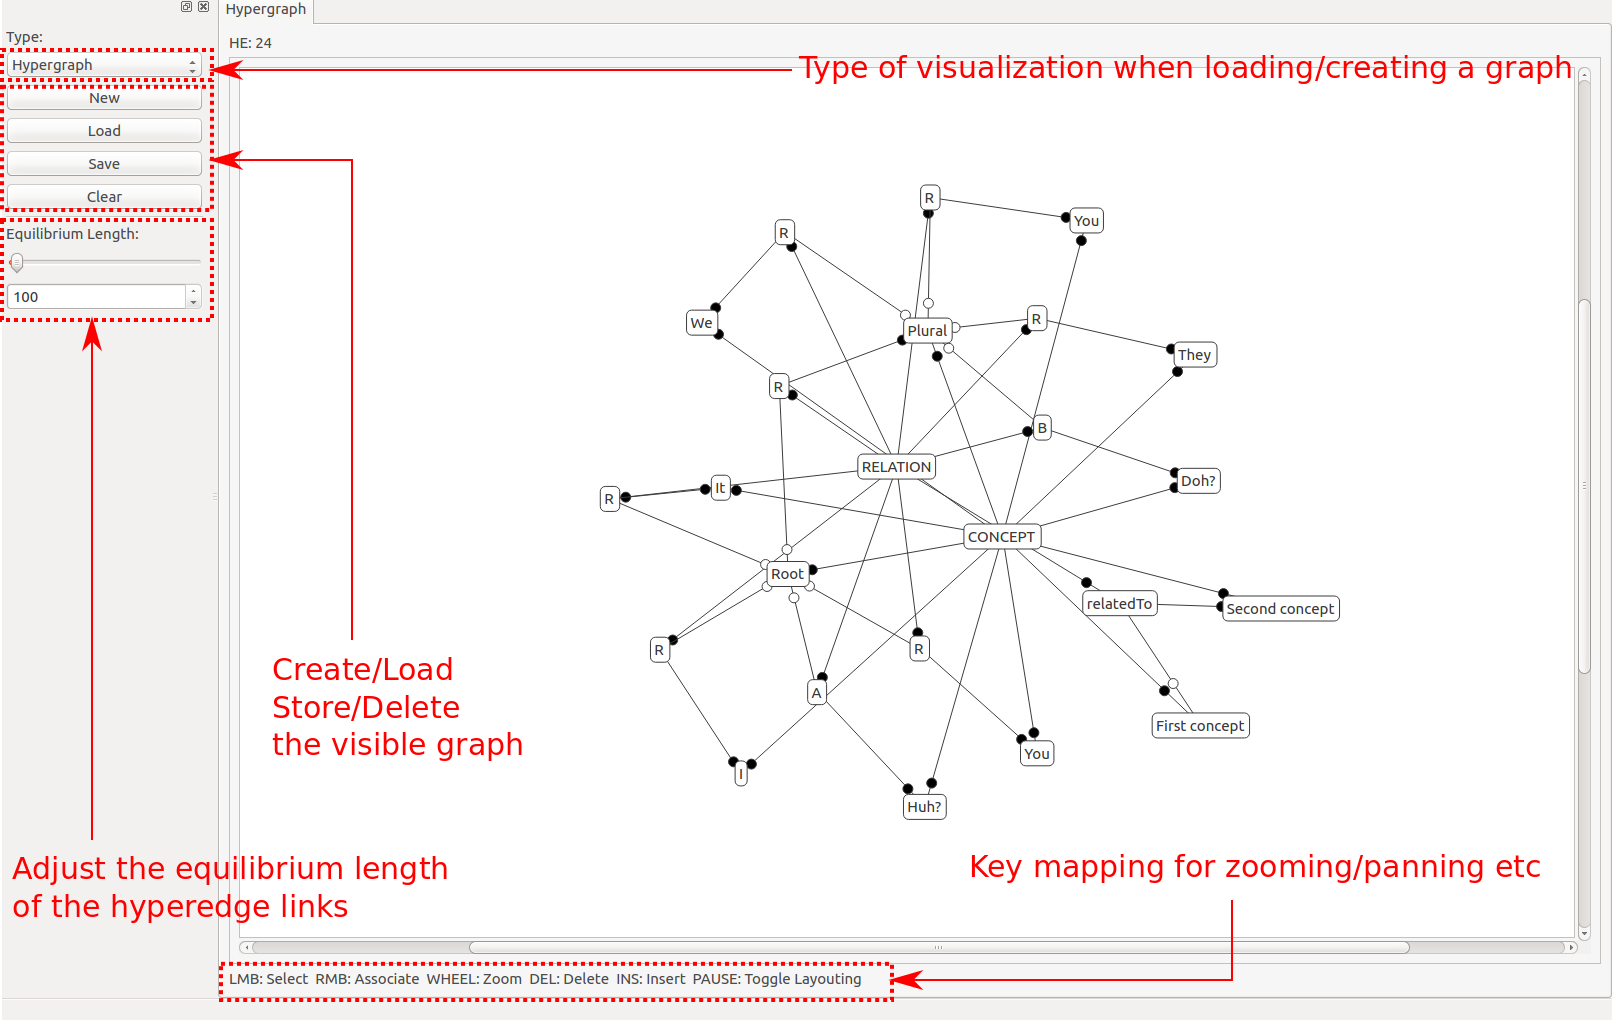
\includegraphics[width=\textwidth]{pics/HypergraphGUI.png}
\end{frame}

% Insert
% * Common Concept Graph Viz
\begin{frame}{Different Visualization}
    \begin{columns}
    	\begin{column}{.5\textwidth}
        \centering
        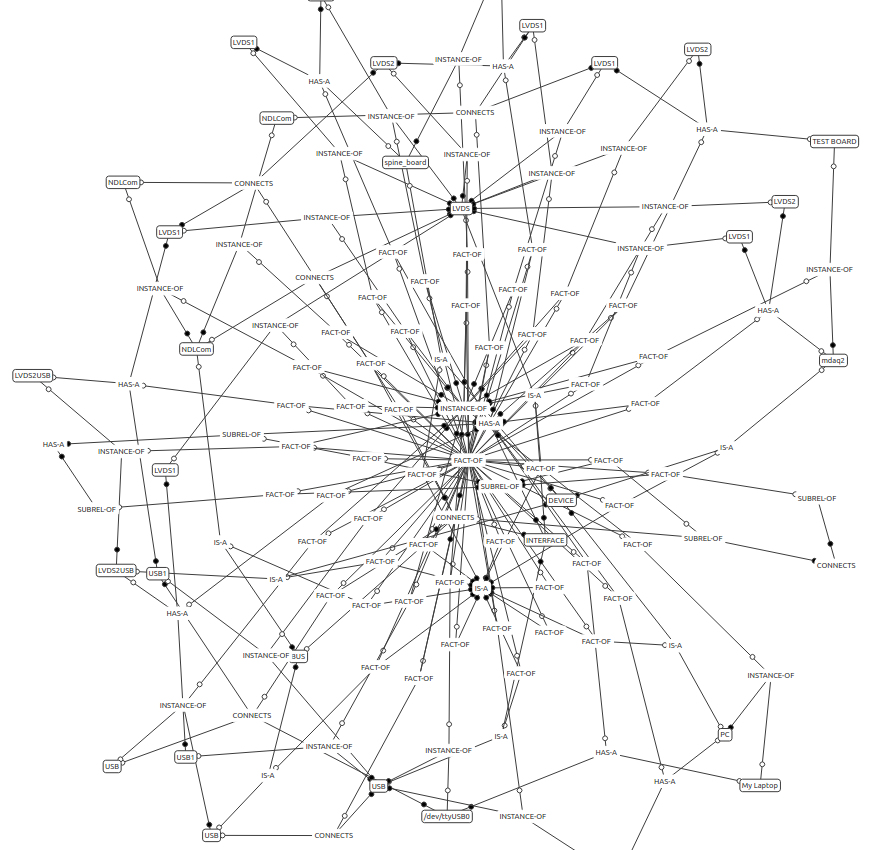
\includegraphics[width=\textwidth]{pics/HardwareGraph.png}
    	\end{column}
    	\begin{column}{.5\textwidth}
        \centering
        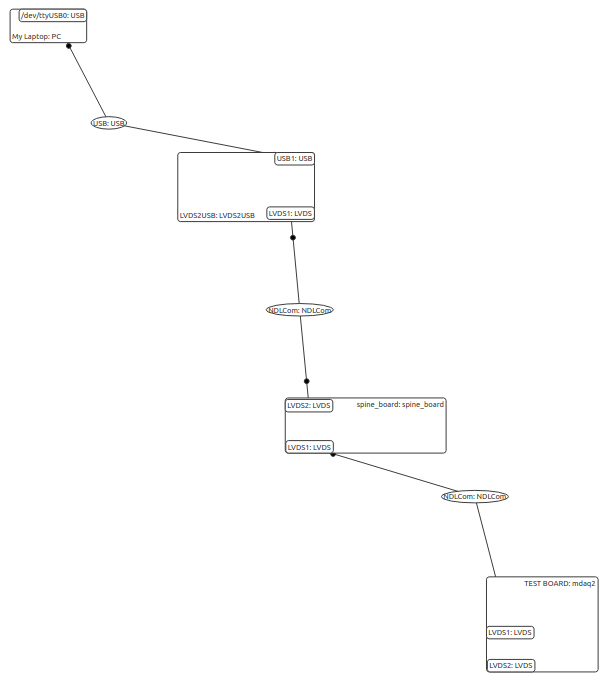
\includegraphics[width=\textwidth]{pics/HardwareGraphInterpreted.png}
    	\end{column}
    \end{columns}
\end{frame}

% * Skeleton generators
% * Insert pattern matching
\begin{frame}{Pattern Matching}
    \centering
    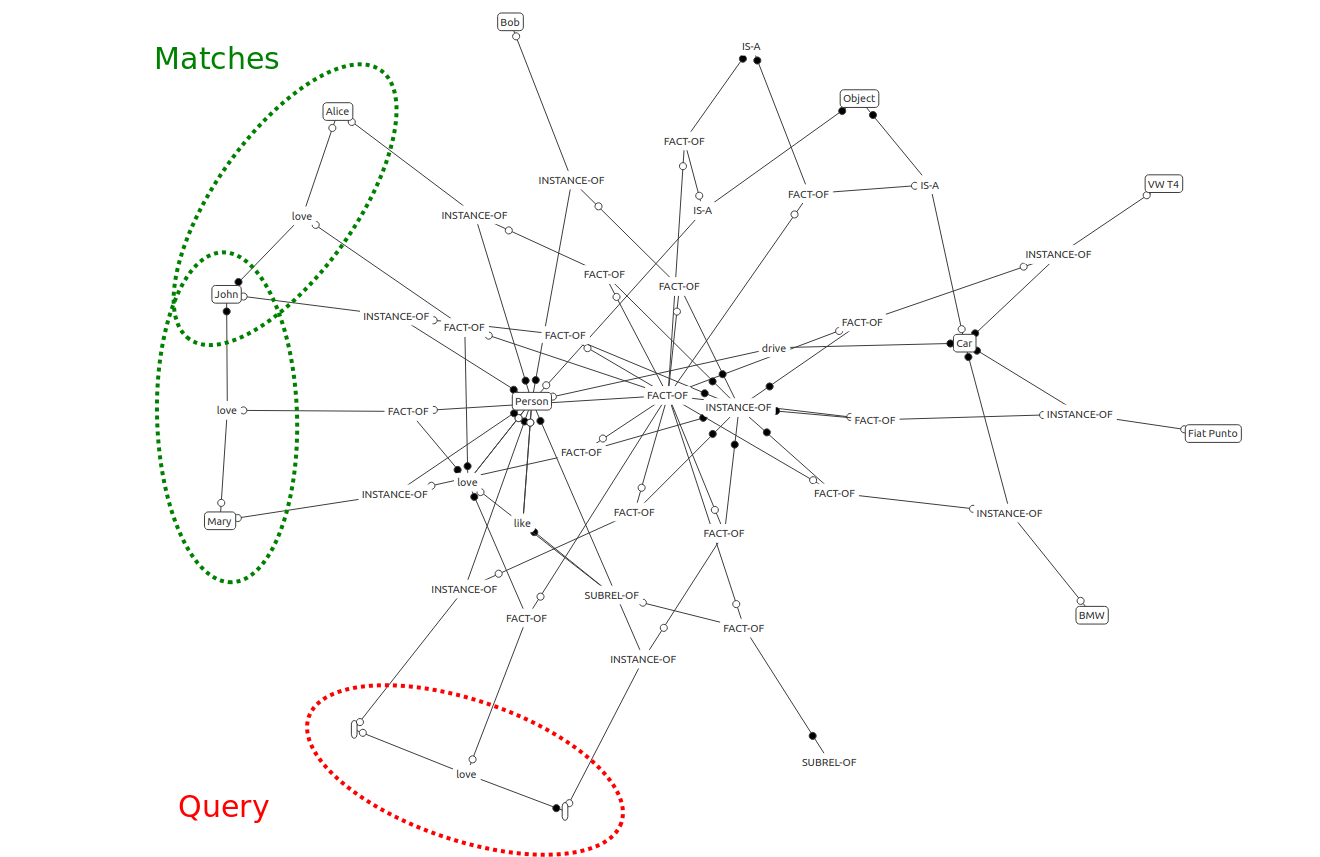
\includegraphics[width=\textwidth]{pics/QueryGraphModified.png}
\end{frame}


%%% SUMMARY & OUTLOOK %%%

\begin{frame}{Status}
    \begin{columns}
    	\begin{column}{.5\textwidth}
    		\begin{itemize}
    		\item[+] Generalized hypergraph library
    			\begin{itemize}
    			\item[+] Import/export from/to YAML
    			\item[+] Unique identifier handling
    			\item[+] Hyperedge operators (union,intersect,subtract)
    			\item[+] Hypergraph operators (union)
    			\end{itemize}
            \item[+] Common relation definition
    		\item[+] Hypergraph GUI to build/load/store hypergraphs
            \item[+] Graph traversal for transitive closure
            \item[+] Pattern matching for queries
    		\end{itemize}
    	\end{column}
    	\begin{column}{.5\textwidth}
    		\begin{itemize}
            \item[-] Domain specification rules
    			\begin{itemize}
                \item[-] Positive/negative matches
                \item[-] Graph rewriting
    			\end{itemize}
            \item[-] Missing domains
    			\begin{itemize}
                \item[-] Electrical domain
                \item[-] Mechanical domain
                %\item[-] Implementation domain
                %\item[-] Algorithm $\cup$ Implementation
                \item[-] Device $\cup$ Implementation
                \item[-] Algorithm $\cup$ Device
    			\end{itemize}
    		\item[-] Feature complete generators and workflow
    		\end{itemize}
    	\end{column}
    \end{columns}
\end{frame}


\begin{frame}{Outlook}
    \begin{itemize}
    \item Domain specification rules using pattern matching and conditional graph rewriting\\
          Idea: Positive Match m, Negative Match n: If $m \cap n = \emptyset$, apply rule to transform $m \to m^{'}$
    \item Feature complete generators for e.g. skeleton code\\
          Basic implementations exist already
    \item Database backend for storage/retrieval\\
          Idea: YAML + GIT, BerkeleyDB
    \item Tools to build deployments
    \end{itemize}
\end{frame}

\begin{frame}[plain]
    \begin{center}
        \huge
        Thank you. Any questions?
    \end{center}
\end{frame}

\end{document}
